%!TEX root = pfc-memoria.tex
%!TEX encoding = UTF-8 Unicode

\part{Introducción y objetivos}

\chapter{Introducción}

\chapter{Objetivos del proyecto}

\chapter{Estructura de la memoria}

\part{Estudio de viabilidad}

\chapter{Metodología de trabajo}

\chapter{Planificación temporal}

\chapter{Análisis del esfuerzo de desarrollo}

\part{Desarrollo del proyecto}

\chapter{Análisis de requisitos}

\resizebox{0.5\textwidth}{!}{\input{diag1.puml}}

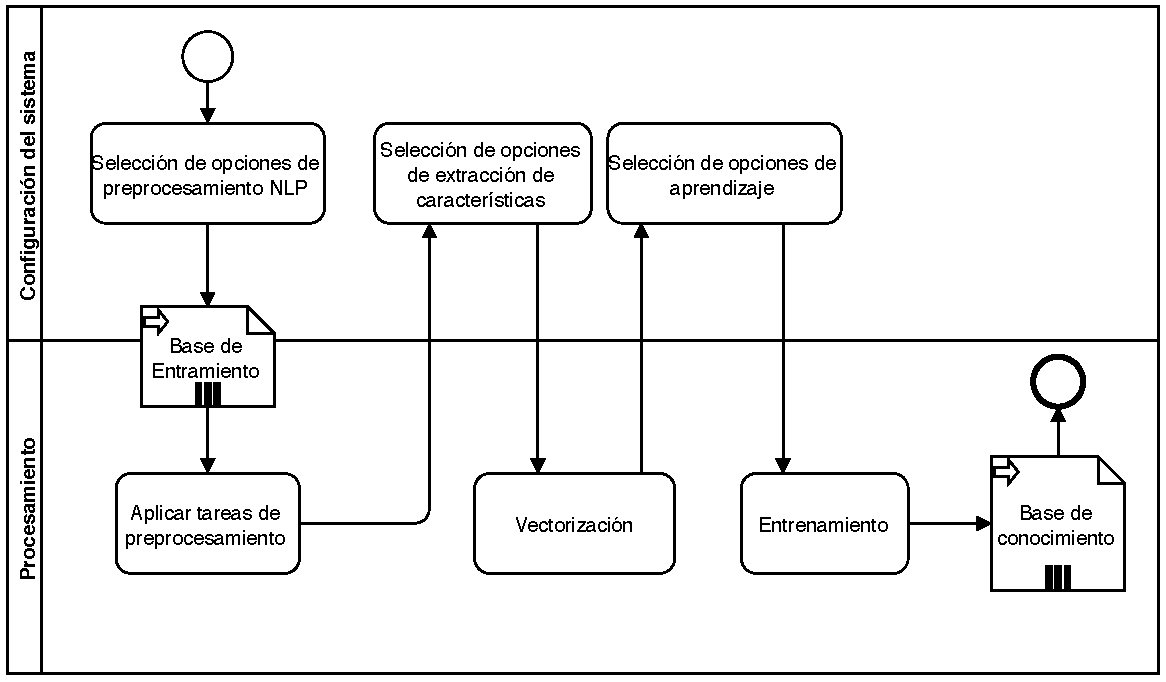
\includegraphics[width=\textwidth]{bpmn-entrenamiento}



\chapter{Diseño del sistema}

\chapter{Implementación}

\section{Rendimiento en Python}

Se observó que la carga del modelo entrenado \path{GoogleNews-vectors-negative300.bin.gz} consumía mucho tiempo y espacio ($\approx$\si{4.5}{GiB} y unos 5 minutos). Este modelo ha sido publicado por Google en el repositorio del proyecto \code!word2vec! basado en el \emph{dataset} de Google News (aproximadamente 100 mil millones de palabras). El modelo contiene vectores 300-dimensionales para 3 millones de palabras y de frases (bigramas y trigramas). Las frases se obtuvieron usando una aproximación dirigida por datos sencilla, como se encuentra descrito en \cite{DBLP:journals/corr/MikolovSCCD13}.

Por ello se convirtió inicialmente el modelo del \emph{Word2Vec} original en la representación interna provista por \code!gensim!, que soporta en \emph{unpickling} de datos de NumPy, de mejor desempeño.

El procedimiento para la conversión es:

\begin{minted}{python}
from gensim.models.word2vec import Word2Vec
# lectura sin optimizar
model_orig = Word2Vec.load_word2vec_format('GoogleNews-vectors-negative300.bin', binary=True)
# escritura optimizada
model_orig.save('GoogleNews-vectors-negative300.bin.gensim')
\end{minted}

Y para la carga de la versión optimizada:

\begin{minted}{python}
from gensim.models.word2vec import Word2Vec
# lectura optimizada
model = Word2Vec.load('GoogleNews-vectors-negative300.bin.gensim', mmap='r')
\end{minted}


\part{Aseguramiento de la calidad}

\chapter{Plan de pruebas}

\chapter{Plan de mantenimiento}

\part{Conclusiones}

\chapter{Conclusiones}

\part{Apéndices}
\appendix

\chapter{Manual de usuario}

%bibliografía